\documentclass{article}
\usepackage{fontspec}
\usepackage{polyglossia}
\setdefaultlanguage{french}
\usepackage[a4paper,margin=1cm]{geometry}

\usepackage{amsmath}
\usepackage{amssymb}
\usepackage{array}
\usepackage{auto-pst-pdf}
\usepackage{booktabs}
\usepackage{cite}
\usepackage{graphicx}
\usepackage{lmodern}
\usepackage{marvosym}
\usepackage{mathrsfs}
\usepackage{minted}
\usepackage{multicol}
\usepackage{multirow}
\usepackage{paralist}
\usepackage{schemabloc}
\usepackage{siunitx}
\usepackage{soul}
\usepackage{tikz}
\usepackage[european,cuteinductors,siunitx]{circuitikz}
\usepackage{url,hyperref}
\usepackage{verbatim}
\usepackage{xunicode,xltxtra}
\usepackage{color}

\title{
\includegraphics{../../../images/inp-enseeiht} \\ ~ \\ ~ \\ ~ \\ ~ \\ MMIC Tutorial}
\author{François Pierron \& Guilhem Saurel}
\date{\oldstylenums{\today}}

\renewcommand{\thesection}{\Roman{section}}

\begin{document}

\begin{titlepage}
    \setcounter{page}{0}
    \maketitle
    \thispagestyle{empty}
    \tableofcontents
\end{titlepage}


%On commence par trouver le point de polarisation. Pour cela, on se place sur la courbe IDS en fonction de VDS pour VGS = 0, ce qui donne un IDSS de 49mA, et on veut donc atteindre un IDS = IDSS/2 = 24.185 en modifiant VGS. On trouve alors un VGS de -0.26 V.

%Pour la bobine, à 8GHz, S11 est optimal à 6.602 nH.
%Si on ajoute la capa, S11 est minimal à 8GHz à 6.498 nH, et S13 est minimal à 8GHz pour 1.299 pF.
%Cependant, vu que la capa depasse 1 pF, il faut changer son modèle.
%idem, pour 6.497 nH et 3.525 PF.
%Après avoir rajout quelques lignes et tee, 6.134 3.289
%À ce moment là, on va voir sur le truc web, on dit qu’on a un spiral inductor de 6.134nH de 10um / 10um, et paf, la frequence de resonnance est de 8.56GHz, CEQUINEVAPASDUTOUT !
%Du coup on s’en fout, on met deux bobines de 3.067

%NB: c’est plus interessant de mettre les tee sur la couche IN. et OSEF si c’est marque que la couche BE fait 11 en vrai ça fait 10 à la fin du process techno.

%Une fois qu’on a mis deux bobines, faut re-tune: 3.198 2.654 × 2

%On fait alors le circuit complet. Ça se chevauche un poil.

%On passe alors à la stabilite. C’est pas bon du tout, du coup on essaye avec des resistances au pif, sauf que ça rajoute trop de bruit.

%On essaye alors plein de trucs au hasard pendant des heures en essayant de concilier gain, bruit, coefficient de Rollet et coefficient de stabilite. La place prise par les composants est aussi un facteur non negligeable, mais vu les autres contraintes, ce n’est pas notre premier problème. On peut essayer de relacher un peu le cahier des charges, en essayant  d’avoir une stabilite inconditionnelle seulement jusqu’à 30GHz.

%Après de longues divagations, on se rend compte qu’on n’arrive pas à respecter le cahier des charges sur le gain et la stabilit à la fois. On decide alors d’essayer d’augementer le gain au detriment du facteur de bruit, en ajoutant une bobine en parallèle sur la grille. Ça marche, et nous laisse un gain superieur à 11dB, un NFmin de 1.2 et une stabilite limite, mais correcte.

%L’etape suivante consiste à adapter le signal en entre. Pour cela, on trace les cercles de gain et les cercles de bruit, et on s’arrange pour trouver un point qui concilie le mieux possible ces deux aspects. On choisi un gain de 10.5 dB pour un bruit de 1.43.
%On note alors l’impdance du point qui correspond, puis, grace à l’outil SmithChart, on trouve la valeur de la capacite serie et de la bobine parallèle à ajouter en entree du montage pour obtenir cette impedance et donc ce couple gain/bruit.

%On fait alors la même chose en sortie, et puis on regarde les paramètres S.

%Et là, c’est le drame.

%On recommence.

%cible           => theorique       => tune
%1.525 + 0.647 j => 1.36nH \& 444 fF => 1.176 nH \& 370 fF
%2.487 - 1.865 j => 4.1 nH \& 233 fF


%On recommence, en repartant du circuit avec juste les machins DC pour essayer de partir avec un maxgain plus fort

%1.727 - 0.528 => 2.93 nH 422 fF

%2.16 358
%2.13 281

%1.43 310


%sortie

%1.04 394

%FIN
%3.7839 nH
%3 nH

%--------- results
%1157 x 967 um
%les sources consomment 0.28 x 20.85 et 3 x 244.8 mW

\begin{centering}

\section{Rappel du cahier des charges}

\begin{tabular}{|c|c|c|c|}
    \hline
    \textbf{Parametres} & \textbf{Spécifications} & \textbf{Remarques} & \textbf{Priorité} \\
    \hline
    Bande passante & 7.9 -- 8.1 GHz & & 1 \\
    \hline
    Gain & >10dB & sur la bande de fréquence & 1 \\
    \hline
    Variation du gain & < 0.2dB & sur la bande de fréquence & 2 \\
    \hline
    Figure de bruit & < 1.5dB & & 1 \\
    \hline
    Adaptation en entrée/sortie & <-20dB & <-25dB cible & 2 \\
    \hline
    Consommation DC & & TBD & 2 \\
    \hline
    Stabilité & Inconditionnelle & 0--60GHz & 1 \\
    \hline
    Point de compression à 1dB & & TBD & 2 \\
    \hline
    Taille des pattes DC & 150 x 100 \si{\micro\meter} & & 1 \\
    \hline
    Entrée/Sortie RF & lignes axiales & & 1 \\
    \hline
    Accès de polarisation & VGS et VDS: haut & & 1 \\
    \hline
    Pourcentage de puces avec un NF<1.8dB & cible:>80\% & & 2 \\
    \hline
    Critères de linéarité: IP3, C/I3 & & TBD & 3 \\
    \hline
\end{tabular}

\newpage
\section{Calcul du point de polarisation}

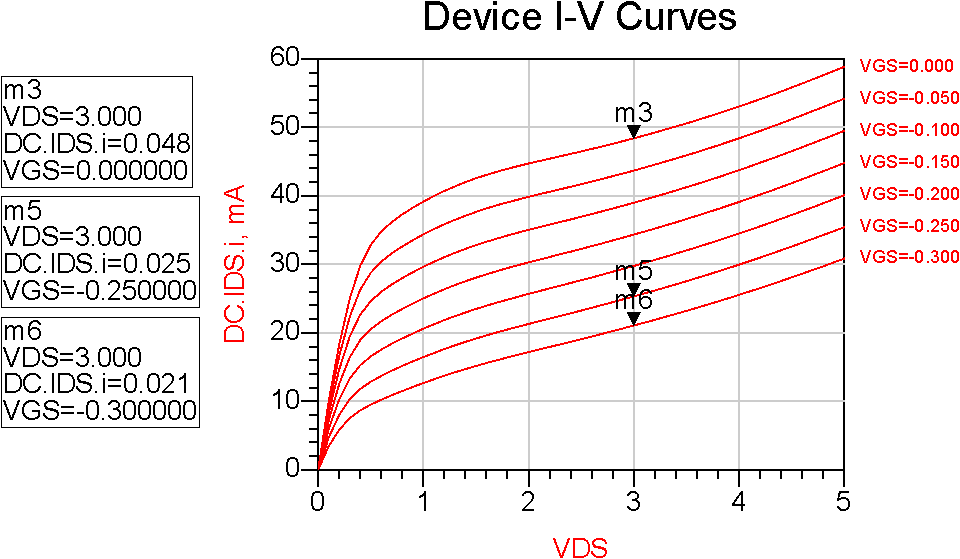
\includegraphics[width=\linewidth]{polar.png}

On doit donc choisir un $V_{GS}$ entre -0.25V et -0.3V.

\newpage
\section{Stabilité, gain maximal, figure de bruit minimale, et cercles de gain et de bruit}
\subsection{Stabilité}

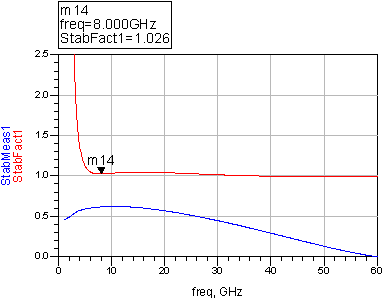
\includegraphics{stab.png}

\subsection{Gain Maximal}

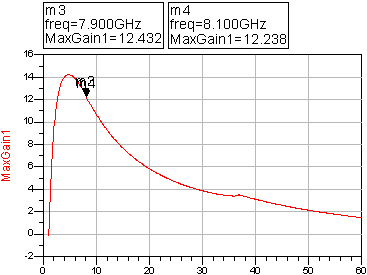
\includegraphics{gain.png}

\subsection{Figure de bruit minimale}

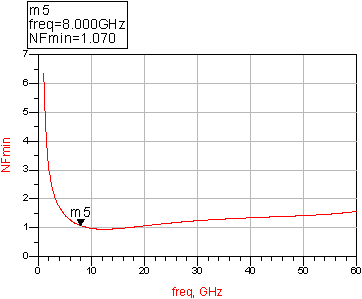
\includegraphics{nf.png}

\subsection{Cercles de gain et de bruit}

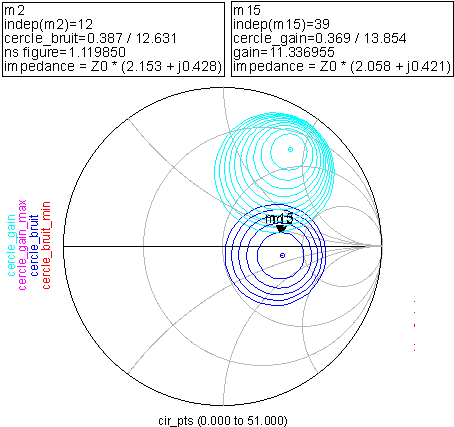
\includegraphics{cercles.png}

\newpage
\section{Résultats Finaux}
\subsection{Figure de bruit finale}

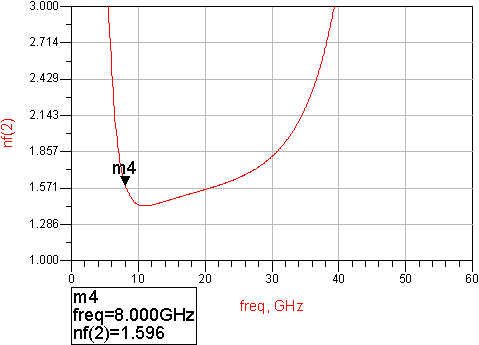
\includegraphics{nf_end.png}

\subsection{Paramètres S finaux}

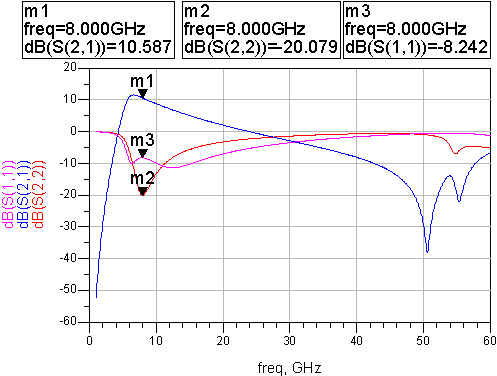
\includegraphics{Sparam.png}

\subsection{Stabilité finale}

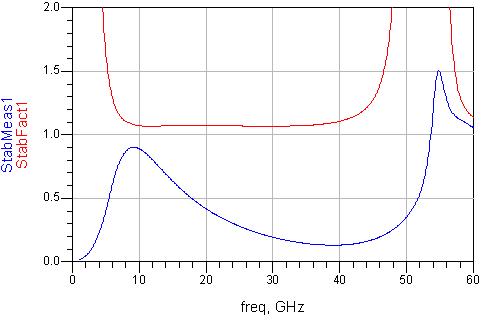
\includegraphics{stab_end.png}

\subsection{Variations du gain sur la bande de fréquence}

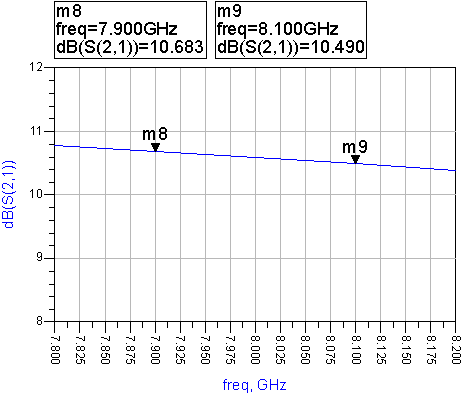
\includegraphics{variation.png}

\section{Circuit final}
\subsection{Schéma simplifié}

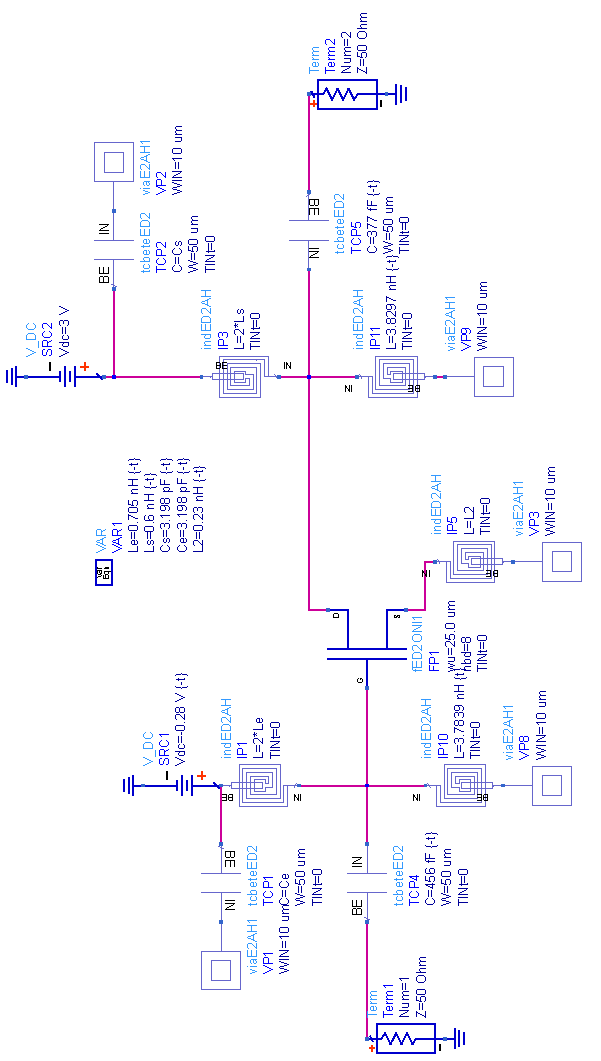
\includegraphics[width=14cm]{simpli_schema.png}

\subsection{Layout}

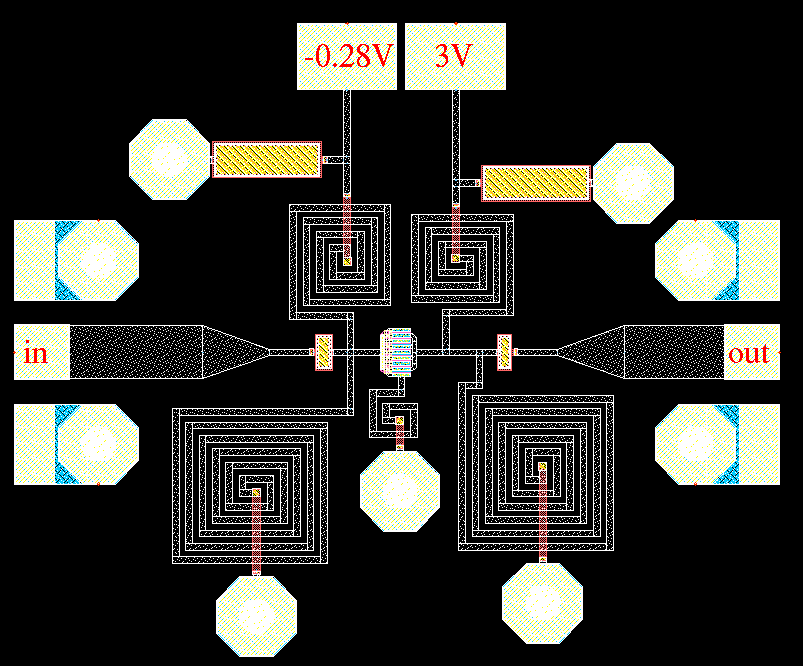
\includegraphics[width=\linewidth]{layout_fini.png}

Ce layout tient sur 1157 x 967 \si{\micro\meter}

\newpage
\section{Retour sur le cahier des charges}

\begin{tabular}{|c|c|c|c|c|}
    \hline
    \textbf{Parametres} & \textbf{Spécifications} & \textbf{Remarques} & \textbf{Résultat} \\
    \hline
    Bande passante & 7.9 -- 8.1 GHz & & \\
    \hline
    Gain & >10dB & sur la bande de fréquence & \textcolor{green}{10.5dB} \\
    \hline
    Variation du gain & < 0.2dB & sur la bande de fréquence & \textcolor{green}{0.19dB} \\
    \hline
    Figure de bruit & < 1.5dB & & \textcolor{orange}{1.59} \\
    \hline
    Adaptation en entrée/sortie & <-20dB & <-25dB cible & \textcolor{green}{<-20} en sortie et \textcolor{red}{-8} en entrée\\
    \hline
    Consommation DC & & TBD & $0.28 \times 20.8 + 3 \times 245 = 741 \si{\milli\watt}$\\
    \hline
    Stabilité & Inconditionnelle & 0--60GHz & \textcolor{green}{OK} \\
    \hline
    Point de compression à 1dB & & TBD & \textcolor{red}{N/A} \\
    \hline
    Taille des pattes DC & 150 x 100 \si{\micro\meter} & & \textcolor{green}{OK} \\
    \hline
    Entrée/Sortie RF & lignes axiales & & \textcolor{green}{OK} \\
    \hline
    Accès de polarisation & VGS et VDS: haut & & \textcolor{green}{OK} \\
    \hline
    Pourcentage de puces avec un NF<1.8dB & cible:>80\% & & \textcolor{red}{N/A} \\
    \hline
    Critères de linéarité: IP3, C/I3 & & TBD & \textcolor{red}{N/A} \\
    \hline
\end{tabular}


\end{centering}

\end{document}

